
In the \wbx\ analysis no significant excess of data over the 
expected background has been observed in the \mreco\ spectrum
of Figure~\ref{fig:mrecoTIGHT}.
The observed and expected upper limits on the \TTbar\ production cross section 
times branching fraction as a function of $m_{\T}$ are shown in 
Figure~\ref{fig:limits1D_wbx} for the two chosen benchmark scenarios,
namely the chiral model with 100\% BR($T\to Wb$) and the weak-isospin singlet 
model.
All results include both statistical and systematic uncertainties,
and the consistency of the data with the background prediction is 
assessed following the concepts presented in Section~\ref{sec:cls}
by computing the $p$-value under the background-only hypothesis
(1-$CL_{\rm b}$) for each point of the two-dimensional plane 
(each point corresponding to a signal scenario) and for every heavy 
quark mass point considered (one two-dimensional plane is built for each
$m_T$ value). The smallest $p$-value found is of 0.095 for a vector-like
top-partner with mass $m_{\T}=350\gev$, $BR(\T \to Zt)=0.9$ 
and $BR(\T \to Wb)=BR(\T \to Ht)=0.05$, which corresponds to a 
significance of 1.7 standard deviations above the 
background-only prediction, which is, therefore, not significant.
For a chiral fourth-generation $\T$ quark, an observed (expected) 95\%  CL  limit 
$m_{\T}>740\,(770)\gev$ is obtained for the central value of the 
theoretical cross section.
This result can also be applied to a $Y$ vector-like quark with electric charge of
$-4/3$ and decaying into a $W^-$ boson and a $b$ quark.
For a vector-like singlet $\T$ quark, an observed (expected) 95\%  CL  limit 
$m_{\T}>505\,(630)\gev$ is obtained for the central value of the 
theoretical cross section.

%To assess the impact of the systematic uncertainties on the limit,
%the result has been compared with what is obtained including in the
%analysis only the statistical errors and it was found that systematic
%uncertainties give a degradation of the expected cross section
%limit by $\sim$50\% for the higher $m_{\T}$ values used.
\begin{figure}[h!tb]
\begin{center}
\subfigure[]{\label{fig:limits1D_wbx_chiral}
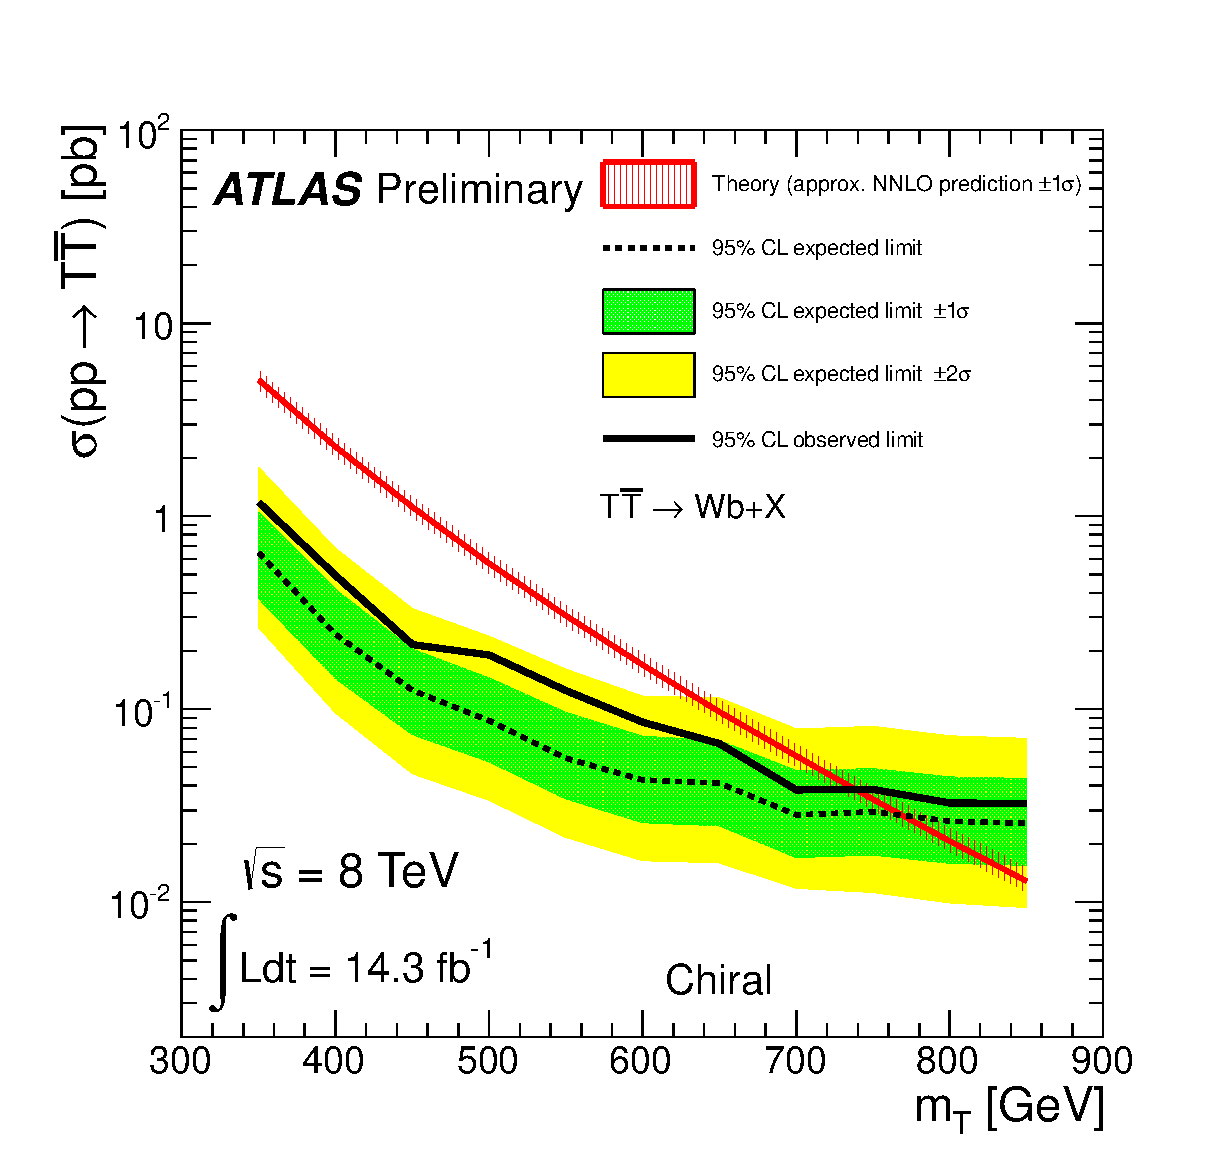
\includegraphics[width=0.45\textwidth]{results/figures/NewttbarMod/lim_chiral_bin1_WbX.eps}}
\subfigure[]{\label{fig:limits1D_wbx_singlet}
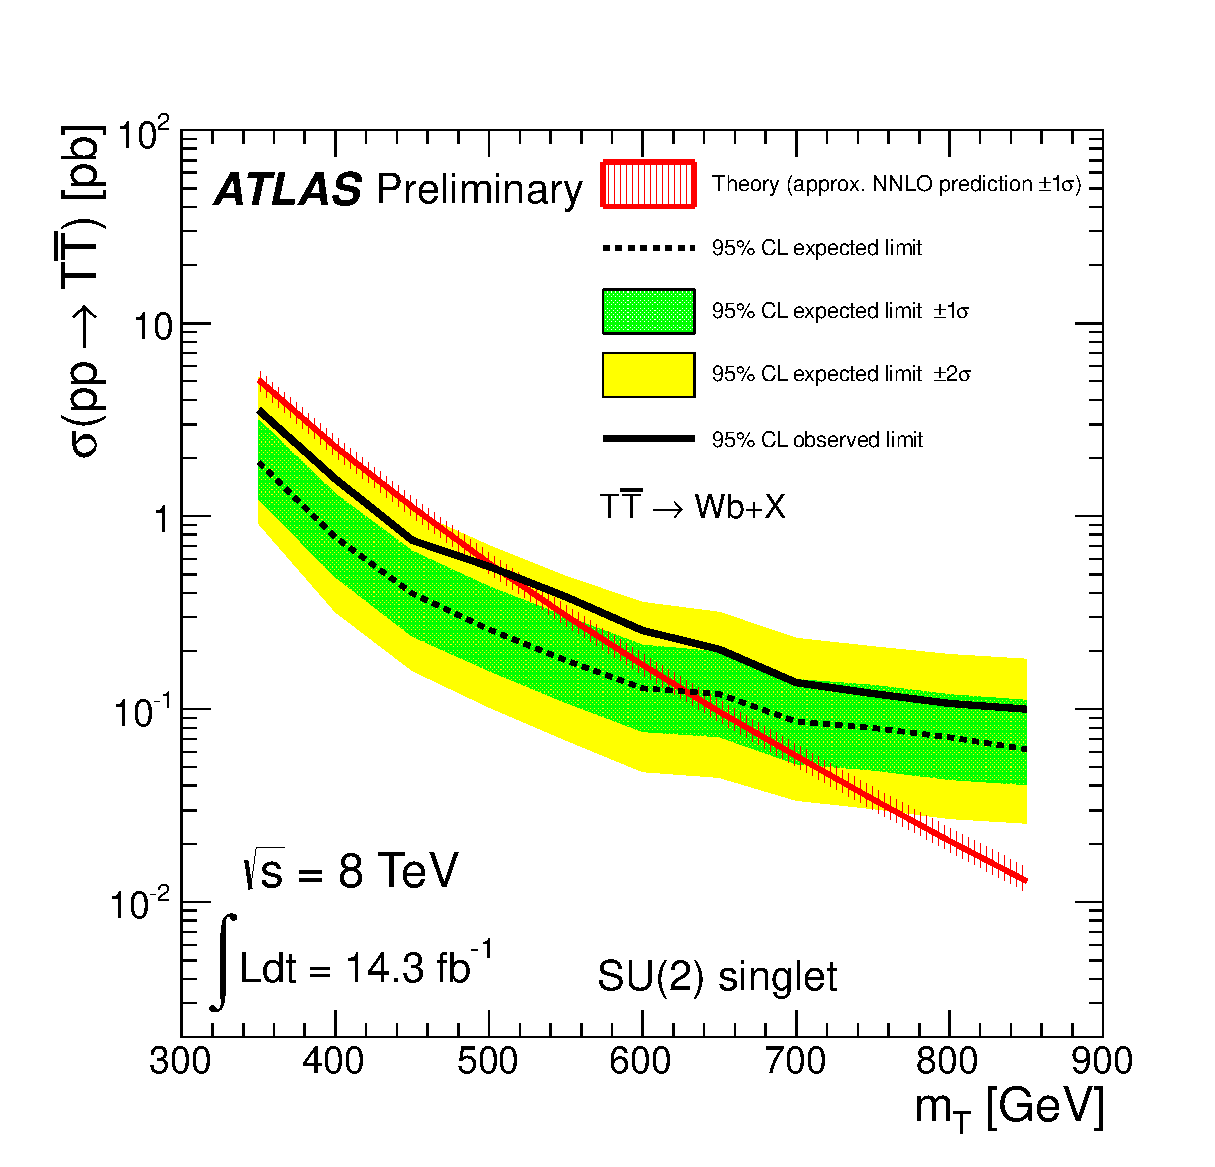
\includegraphics[width=0.45\textwidth]{results/figures/NewttbarMod/lim_singlet_bin1_WbX.eps}}
\caption[bla]{Observed (solid line) and expected (dashed line) 95\% CL upper limits on the $\T \bar{\T}$ cross section times branching fraction
for (a) a chiral fourth-generation $\T$ quark and (b) a vector-like singlet $\T$ quark  as a function of the $\T$ quark mass. 
The surrounding shaded bands correspond to the $\pm1$ and $\pm2$ standard deviations around the expected limit. 
The thin red line and band show the theoretical prediction and its $\pm1$ standard deviation uncertainty.

\label{fig:limits1D_wbx}}
\end{center}
\end{figure}


Concerning the quasi-model independent strategy, 
we recall here that in the two-dimensional plane the gray area
corresponds to the unphysical region where the sum of BRs
exceeds unity. In every plane two benchmark models are indicated
as a plain circle and star symbols, corresponding respectively to the
weak-isospin singlet and doublet scenario BRs values as computed by the
\texttt{PROTOS} event generator.
To probe the full plane the signal samples are reweighted by the ratio
of desired branching ratio to the original branching ratio generated
by \texttt{PROTOS} and the complete analysis are repeated in each point.
The  95\% CL exclusion limits  obtained in the scan of the two-dimensional
plane by varying the mixing of the three decay channel contributions for
different values of $m_{\T}$ are shown in Figure~\ref{fig:limits2D_wbx}. 
This plot reads as follow: taking for instance the $600\gev$ 
vector-like top partner, a heavy quark with
$BR(\T\to W b)>0.7$ is excluded at $\geq 95\%$ CL, 
regardless of the value of the vector-like quark branching ratios to $Ht$ and $Zt$.  
%All the decay modes contribute to the final sensitivity when setting limits.
%For example, assuming $m_{t^\prime}=600\gev$, 
%the acceptance times efficiency of the {\sl tight} selection is 2.45\%, 0.64\%, 0.47\%, 0.10\%, 0.18\% and 0.16\%, for 
%decays to $WbWb$, $WbZt$, $WbHt$, $ZtZt$, $ZtHt$ and $HtHt$, respectively.


\begin{figure}[h!bt]
\begin{center}
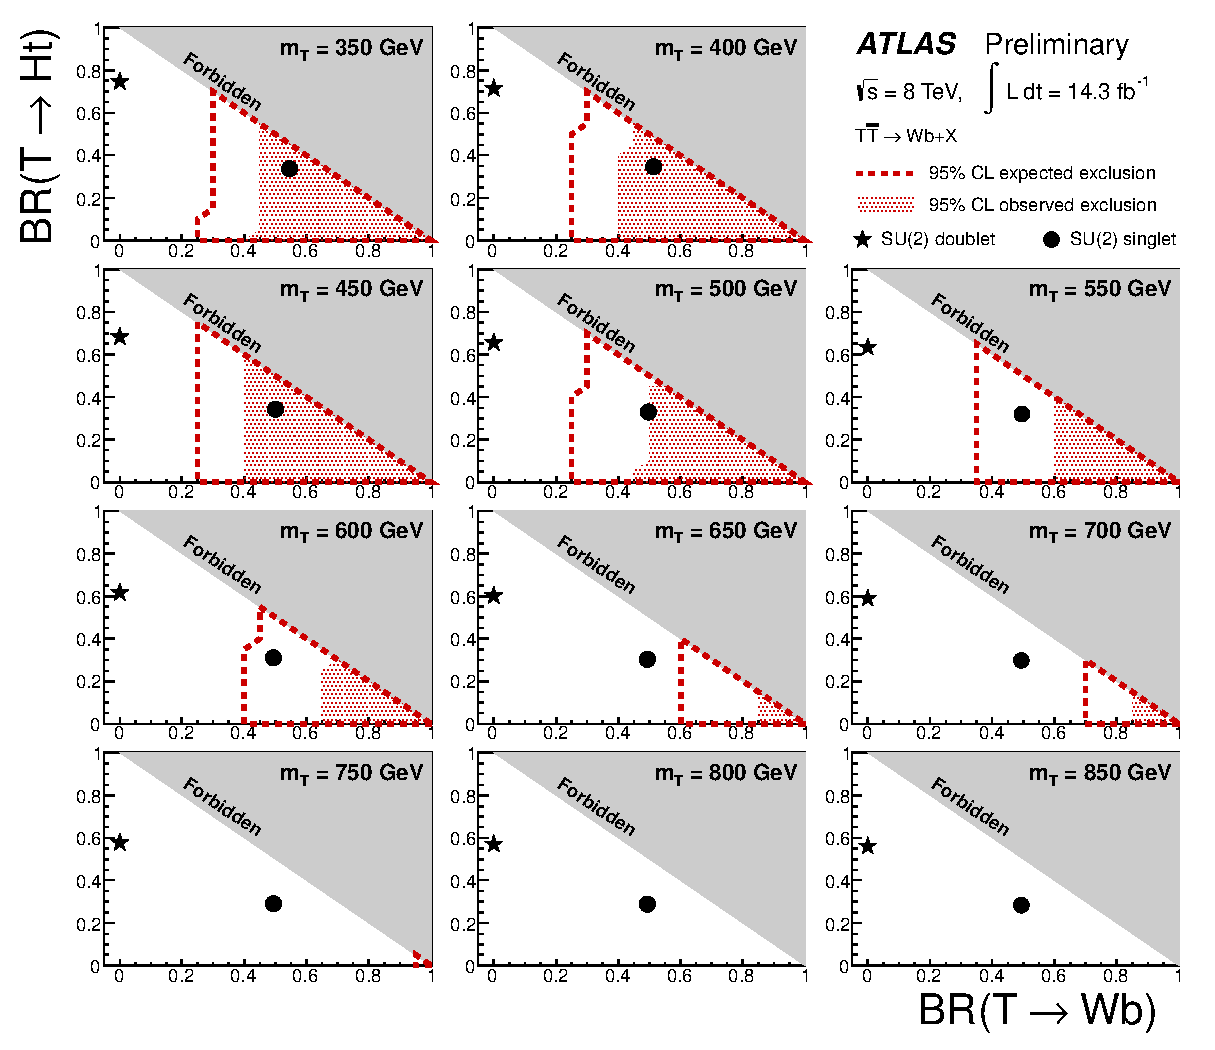
\includegraphics[width=0.9\textwidth]{results/figures/NewttbarMod/lim_Scan2D_tight_Bin1.eps}
\caption{
Observed (red filled area) and expected (red dashed line) 95\% CL exclusion in the plane of
$BR(\T \to Wb)$ versus $BR(\T \to Ht)$, for different values of the vector-like $\T$ quark mass.
\label{fig:limits2D_wbx}}
\end{center}
\end{figure}



